% 4.  Validazione e prestazioni (validazione ?)
% prestazioni: far vedere le ottimizzazioni perchè le api siano veloci 
% usare i grafici sul ridimensionamento della ram
% le api devono rispondere in 29 secondi (mostrare la parte dei metadati che ci metteva troppo tempo per le lookup) era una mappa usata per semplificare la lookup
% requisiti tecnologici -> lambda dura al max 15 minuti
% ottimizzazioni della fase di import (optional)
% * metodologia seguite (?)


\chapter{Performance and Validation}
No performance requirements were established in the specifications provided for the development of the Data Entry Tool. However, since the project is based on the concept of Serverless, which, as mentioned in Chapter 2, means that resources are used on-demand and paid for based on usage, what we could do was optimize their use.
\section{Implementation enhancements}
One of the features that we improved was the API that retrieves the metadata for the dynamic creation of the tables for the end user.

The \code{/metadata} API not only retrieves information about the table and their permissions, but also collects all the fields that will be used to build the table. Of these fields, those with an \emph{External Enum} datatype represent a list of possible values extracted from a lookup table, also recorded in the Tool. An example of this type of field can be seen in Figure \ref{fig:types}. These values represent the relationship between the tables as they are in effect foreign keys. Since the list of possible values for foreign keys is necessary for the proper construction of the table, and for any record addition or update, it means that, for each field representing a foreign key it is necessary to collect all possible values that can be used to refer to a record in the lookup table. 

To collect the possible values for each External Enum field, you must query the source database of the lookup table to retrieve the set of values. It goes without saying that as the number of foreign keys for a table increases, the number of queries increases, and each query requires a connection to the database, which can increase the latency and therefore the waiting time for the creation and use of the table by the end user. This is all considering a single end user of the Tool; with multiple users, the situation is multiplied.

One improvement that I made, described in Section \ref{Knex}, was reusing a previously created connection to a database instead of creating a brand new one every time. However, this shrewdness does not resolve the problem entirely, because it does not take into account either the amount of time needed by the database to actually perform the query, or the latency of the network where the information passes through. Network latency depends on where the databases are located relatively to the datacenter where the Data Entry Tool resides, while the time required for the database to complete the query processing depends on the amount of data to retrieve and the computing capabilities of the hosting machine. In addition, the API Gateway that routes requests to the appropriate Lambda function limits its duration to 29 seconds. This means that if the data cannot be retrieved in this time frame, an operation timeout will be returned to the user. This is an inherent limitation of AWS API Gateway that ensures a near real-time experience for applications using it. However, in these 29 seconds, the same Lambda function can accept multiple requests from the same or different users, optimizing its execution by not tying it to a single user.

\section{Cost-dependent performance}
Taking into account the timing that cannot be controlled by the Tool, what I could do was run the queries in parallel to gather the data. 
However, performing parallel requests to retrieve the data requires a certain amount of CPU power.
As mentioned earlier, resources are used on-demand and paid for based on usage, and by default Lambda functions are set to use a default amount of resources. This can reduce the expense, but also the computational performance of the function. 

AWS Lambda functions are charged monthly based on \textbf{number of requests} and \textbf{duration}, which is the code execution time. A request is represented by the moment when the code starts running in response to an event, which in our case comes from the Gateway API, and AWS Lambda charges the total number of requests across all the functions used. Instead, the duration is calculated on the time interval from when the code start executing until it returns or is terminated, rounded to the nearest upper 100 milliseconds. This means that 100 milliseconds of execution is charged even if it takes less than that. The final price of the Lambda function depends on the amount of memory (RAM) allocated to the function; furthermore, the computational power associated with the function depends linearly on the allocated memory. 
The final price calculation is composed of the sum of the monthly compute charges with the monthly request charges.

\[Request Charges =  \rho * \sigma\]
\[Compute Charges =  \rho * \alpha *\frac{\gamma}{\SI{1024}{\mega\byte}}*\chi \]
\[Total Monthly Charges =  Compute Charges + Request Charges\]

\begin{itemize}
    \item \textbf{\textrho} → requests per month.
    \item \textbf{\textsigma} → price per million of requests.
    \item \textbf{\textalpha} → average Lambda function execution time in seconds.
    \item \textbf{\textgamma} → amount of RAM provided in MegaByte.
    \item \textbf{\textchi} → price per GigaByte used in a second.
\end{itemize}

Let us say, as an example, that the Lambda function that retrieves metadata receives one million requests in a month (\textrho) at a per-million price of \$0.20 (\textsigma), has an average execution time of one second (\textalpha), and \SI{1024}{\mega\byte} of RAM provided (\textgamma) at a price of \$0.000016667 (\textchi) per GB used in one second. With this data we can see that in one month AWS would charge \$16.86 just for this function alone.

Knowing how AWS Lambda charges for its usage, we can take the amount of memory as a variable and see how much its variation affects computational performance, thus determining the execution time of the Lambda function that collects the metadata. Figure \ref{fig:lambdaTime} shows the trend of the execution time on a sample of requests taken directly from the AWS console of the Lambda function to avoid latency due to connection, API Gateway and Lambda Authorizer. In the figure, we can see the different computational performance as the memory increases. When switching from \SI{512}{\mega\byte} to \SI{1024}{\mega\byte} of RAM, the execution time is almost halved, while doubling it further to \SI{2048}{\mega\byte} or \SI{4096}{\mega\byte} we reach a point of diminishing returns where the performance gain is not such as to justify, respectively, doubling or quadrupling the costs. The Table \ref{tab:lambdaTime} further emphasizes the increase in performance.  

Keeping in mind the balance between cost and computational performance, I decided to allocate an amount of memory equal to \SI{1024}{\mega\byte} to this Lambda function, which deals not only with collecting metadata, but also with performing manipulations on the table data on behalf of the user. Following this logic, I have reduced the computational power of those Lambda functions that do not require many resources to be executed in a performant way. All the functions managed on the Administrator side belong to this category.


\begin{table}[!htb]
  \centering
  \caption{Performance gain by increasing memory.}
  \begin{tabular}{|l|r|r|r|r|} \hline
                  & \SI{512}{\mega\byte}    & \SI{1024}{\mega\byte}     & \SI{2048}{\mega\byte}     & \SI{4096}{\mega\byte}     \\ \hline
    \textbf{MIN}  & \SI{1842,00}{\ms}       & \SI{1,00}{\ms}            & \SI{8,00}{\ms}            & \SI{523,00}{\ms}          \\ \hline
    \textbf{MAX}  & \SI{3364,00}{\ms}       & \SI{1854,00}{\ms}         & \SI{1743,00}{\ms}         & \SI{1249,00}{\ms}         \\ \hline
    \textbf{AVG}  & \SI{2025,83}{\ms}       & \SI{1121,24}{\ms}         & \SI{769,25}{\ms}          & \SI{712,60}{\ms}          \\ \hline
    \textbf{95\%} & \SI{2245,60}{\ms}       & \SI{1437,75}{\ms}         & \SI{1207,15}{\ms}         & \SI{1031,80}{\ms}         \\ \hline
  \end{tabular}
  \label{tab:lambdaTime}
\end{table}

\begin{figure}[!htb]
    \centering
    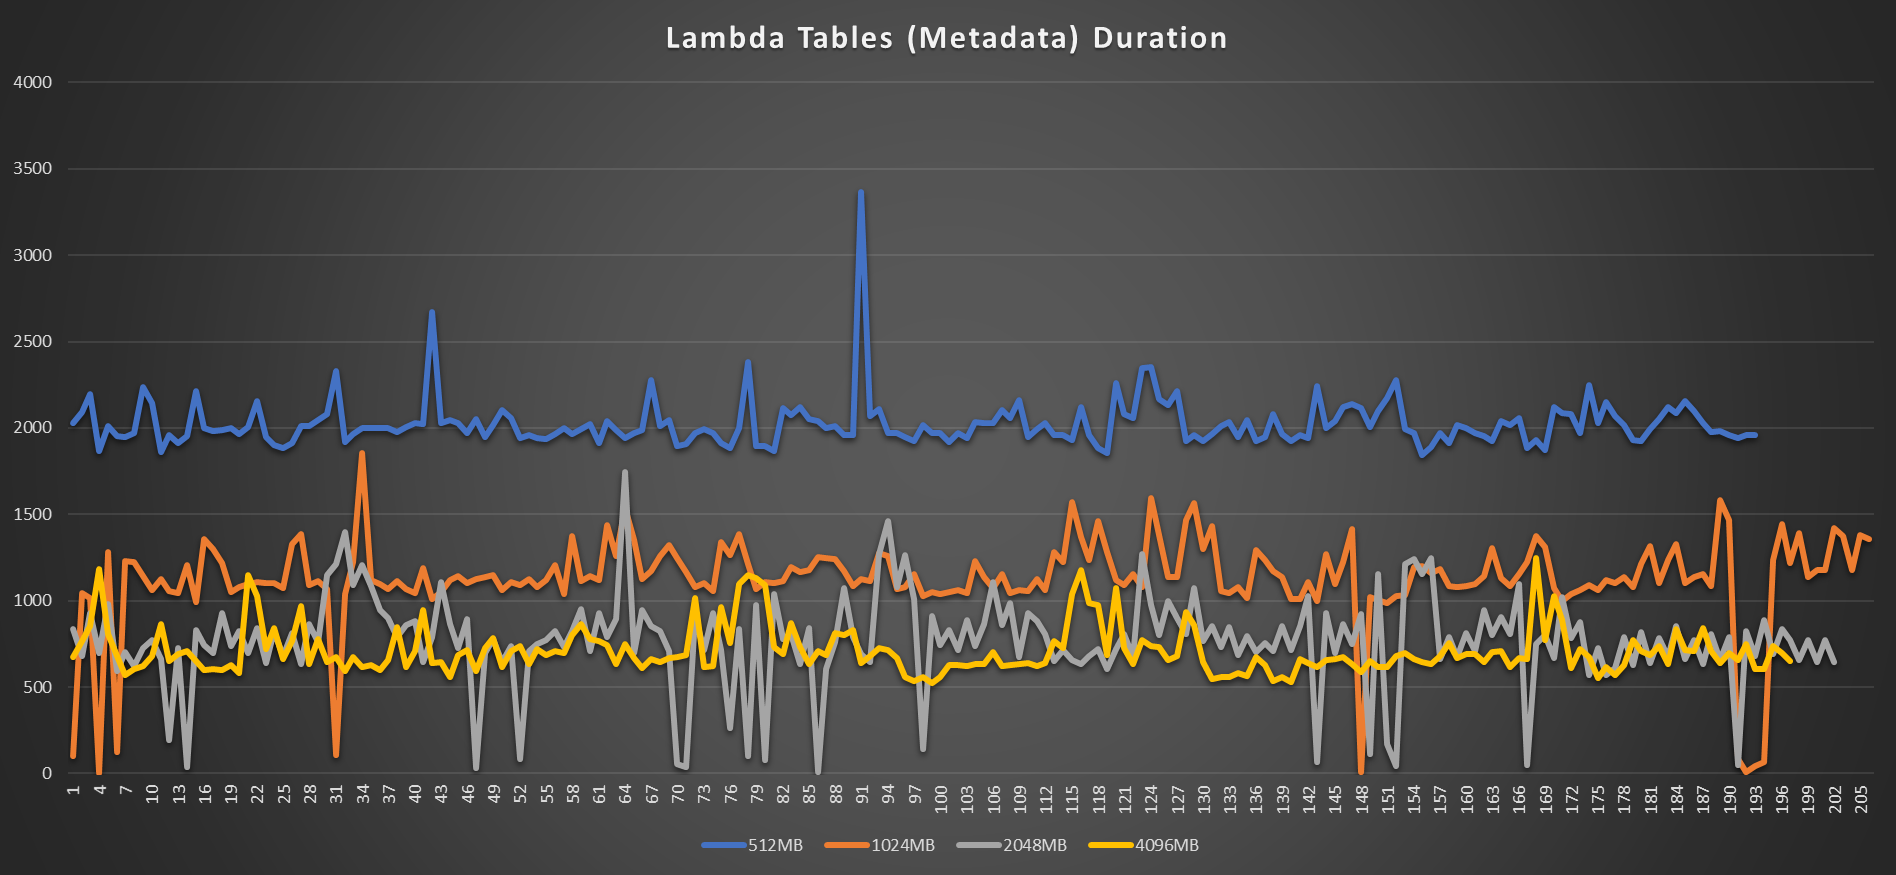
\includegraphics[width=15cm]{chapters/images/ch_4/GetMetadataLambda.png}
    \caption{Lambda execution time based on the memory provided.}
    \label{fig:lambdaTime}
\end{figure}


\section{Validation}
\subsection{Testing during development}
To ensure that the Data Entry Tool met the requirements, it underwent several tests. During the development of the Back-End side, the tests were performed through the use of the Serverless Framework which allows the entire Back-End code to run locally on the development machine. This way there was no need to deploy unfinished APIs in the development environment. The Serverless Framework instantiated a local server, listening on port 3000, to which it attached the APIs, in effect creating a local API Gateway. Lambda functions that are tied to the APIs were run on the local machine, so that it was possible to see the execution steps and logs on the terminal to verify that the function was working as expected.  However, the Aurora instance at the core of the Tool, for both development and production, and all test databases used were hosted in the AWS datacenter.

On the other hand, during the development of the Front-End side of the tool, just like the Back-End, we were running the application locally; however, we were using the versions of the APIs deployed in the development environment as endpoints for the Back-End requests. The tests focused on the correct display of the information received from the Back-End and the correct interaction with the data located in the different types of databases, always taking into account the speed of data display to maintain a near real-time experience.


\subsection{Meeting the requirements}
To ensure that the Data Entry Tool met the expectations of the client company, it was tested through various use cases and underwent the User Acceptance Test. Some of the use cases that have been provided by the client are:

\begin{itemize}
    \item Division of user access according to the given permissions.
    \item Using tables independently of the underlying database.
    \item Using tables with tens of columns with different datatypes.
    \item Loading the Excel file to populate the table.
    \item Logging of every operation.
\end{itemize}

After developing the frontend side of the Data Entry Tool, the project would periodically go through the User Acceptance Test (UAT), where the client would test it to personally verify that everything they had requested was in place, and if there were adjustments or improvements to be made, these would be fixed and resubmitted at the next UAT. This process of reiterating development with UATs was maintained for an additional 2 weeks after delivery of the finished project, as a hypercare period was established in the contract in case of problems.  

% hypercare di 2 settimane
% quanto sviluppato rispetta i requisiti verificandoli con determinati use case

\subsection{Compared to the pre-existing solution}
The pre-existing solution to manipulate data in multiple tables existing in different databases consisted in a web page tailored for each table. This means that every time there was a need to interact with a new table created in a database, the client had to spend some time creating a new web page to interact with directly, without any check either on the datatype or whether there were any constraints to respect. These web pages had no concept of permissions, meaning that any user had indiscriminate access to any table, and could potentially modify its contents improperly. Moreover, since it was not possible to import data by uploading an Excel file to the page for a particular table, they had decided to store these files in a shared directory without updating the corresponding tables, which in many cases had led to inconsistent data.
With the expanding infrastructure the client was experiencing, this ongoing effort and expense of creating web page after web page for each table was no longer sustainable. 

By developing this project as a plug and play solution, the previous problems have disappeared; administrators need just to make a particular database reachable from their private network, register it in the Tool, add the desired tables, and give permissions to a set of users to interact with them. Everything else is taken care of by the Data Entry Tool.
% * risultati ottenuti rispetto agli obiettivi iniziali
    %-> ora il cliente può gestire più db in unica platform
    %-> prima dovevano fare uno sviluppo di una pagina per ogni nuova tabella da gestire
    %  prima era necessario inserire dei file in rete condivisa
    



